\chapter{Experimental Study}
\section{\label{sec:exp}Experiments}
\label{sec:exp}
In this chapter, we validate the performance of our main approach to evaluate Spatial Alarm queries in Obstructed, and compare it with the naive approach. We run all experiments using a computer with Intel Core i5 2.30 GHz CPU and 4GB RAM.


We have used both real and synthetic datasets to evaluate our solution. In case of real datasets, we have used obstacles and point of interests (POIs) of Germany. The obstacle set has 30674 minimum bounded rectangles (MBRs) of railway lines (rrlines). In our experiment we assume obstacles to be presented by MBRs, but our algorithm can handle any type of obstacles.The POI set has 76999 MBRs of hypsography data (hypsogr). We assume datapoints to be endpoints of the hypsography data.In this way the POIs and obstacles are in the same plane which allows us to simulate a real-life scenario. We do not allow intersections between POIs and obstacles, neither do we allow duplicate POIs or obstacles. In case of synthetic datasets we generate the obstacles and POIs from the real datasets using a uniform distribution.
We normalize both real and synthetic dataset in a $10,000 * 10000$ grid. 

In our algorithm, we assume only one type of POIs. However our algorithm can handle multiple type of POIs also. Two separate R-trees have been used to store the POIs and Obstacles in the memory. We simulate the movement of the client in the runtime. Each movement of the client is generated with a 2 second interval, the direction and velocity of the client is randomly generated. The velocity of the client is assumed to be in the range 0 to 40 m/s. We do not allow intersection between a client's movement and an obstacle MBR.We also do not allow the client to move outside the normalized grid.  

In our experiments, we vary the following query parameters: (i) the length of path  travelled by the client, (ii) the query range r (iv) the size of data sets (synthetic data set). Table ~\ref{table:exp_setup} summarizes the parameter values used in our experiments. In all experiments, we estimate I/O accesses and the query processing time to measure the efficiency of our algorithms. In each set of experiments, we run the experiment for 100 queries and present the average result.

\vspace*{10pt}
\begin{table}[htbp]
  \centering

\begin{tabular}{|c|c|c|}  \hline
 %after \\: \hline or \cline{col1-col2} \cline{col3-col4} ...
  Parameter& Values & Default\\
  \hline
  Length of Clients Movement & 100,200,300, 400 & 500 \\
  \hline
  Alarm Range $r$& 50, 100, 150, 200 & 250\\
  \hline
  Synthetic data set size & 5K, 10K, 15K, 20K & - \\
  \hline
\end{tabular}
\caption{Values of different query parameters used in our experiments} \label{table:exp_setup} \vspace{-2mm}
\end{table}


We first present our experiment results for processing spatial alarm queries for naive approach in Section~\ref{subsec:sum},
then we present experimental results for our main approach (Section~\ref{subsec:max}). Finally, in Section~\ref{subsec:cmp}, we compare the results of two approaches.


\subsection{Naive approach}
\label{subsec:sum}
%%TO DO :Write our naive approach experiment evaluation here
%In this section, we present the experimental results for processing $k$GTP queries for aggregate function SUM. For SUM, we name our proposed approach and the naive approach as $kGTPQ_{sum}$ and $kGTPQ-NA_{sum}$, respectively. In the following sets of experiments, we vary group size, the answer set size, query area, and dataset size. When we vary one parameter, we set other parameters to default values as stated in Table~\ref{table:exp_setup}.

%\textbf{\emph{Effect of group size $n$: }}Figure~\ref{graph:sum_g}(a) and ~\ref{graph:sum_g}(b) show I/Os and processing time, respectively, for processing $k$GTP queries using $kGTPQ_{sum}$ and $kGTPQ-NA_{sum}$. We observe that for both algorithms $kGTPQ_{sum}$ and $kGTPQ-NA_{sum}$, I/Os and processing time increase with the increase of the group size $n$. We also observe that in terms of I/Os, our approach $kGTPQ_{sum}$ outperforms the naive approach $kGTPQ-NA_{sum}$ by 2 orders of magnitude. Moreover, the query processing time of $kGTPQ-NA_{sum}$ is on average one and half order of magnitude higher than that of $kGTPQ_{sum}$.

%\vspace*{10pt}

%\begin{figure}[htbp]
 %\vspace{-2mm}
  %\begin{center}
  %  \begin{tabular}{cc}
   %      \hspace{-5mm}
    %  \resizebox{70mm}{!}{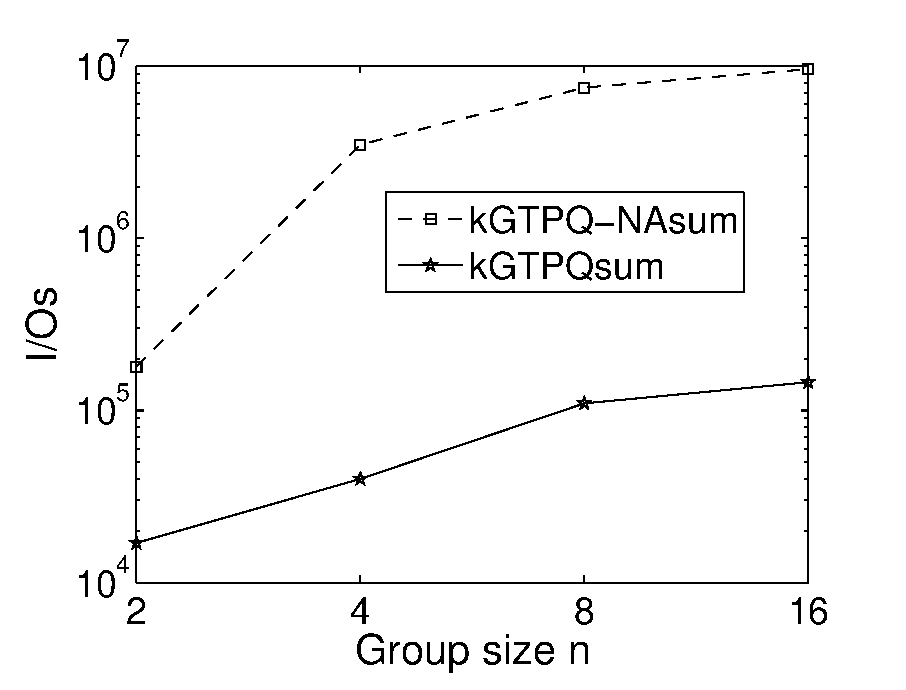
\includegraphics[]{graph/SumGIO.eps}} &
    %    \hspace{-5mm}
     %    \vspace{-2mm}
    %  \resizebox{70mm}{!}{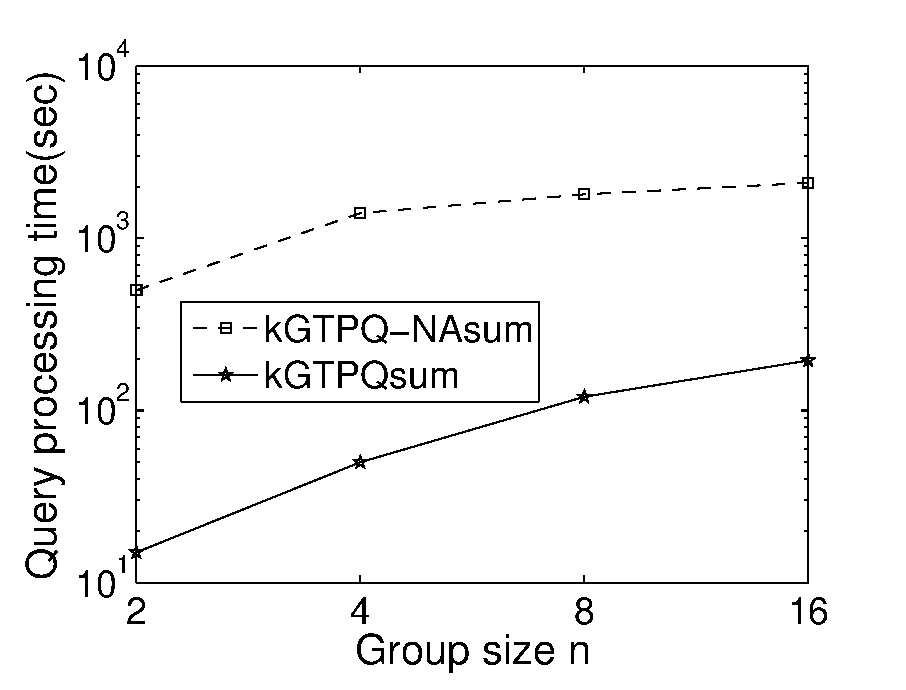
\includegraphics[]{graph/SumGTime.eps}} \\
    %  \scriptsize{(a) \textsc{}\hspace{0mm}} & \scriptsize{(b) \textsc{}}\\
        %\hspace{-5mm}
%        \resizebox{40mm}{!}{\includegraphics{graph/sum/vk_io.pdf}} &
%        \hspace{-5mm}
%      \resizebox{40mm}{!}{\includegraphics{graph/max/vk_io.pdf}} \\
%      \scriptsize{(c) \textsc{sum}\hspace{0mm}} & \scriptsize{(d) \textsc{max}}\\
%      \hspace{-5mm}
%      \resizebox{40mm}{!}{\includegraphics{graph/sum/vk_answer.pdf}} &
%        \hspace{-5mm}
%      \resizebox{40mm}{!}{\includegraphics{graph/max/vk_answer.pdf}} \\
%       \scriptsize{(e) \textsc{sum}\hspace{0mm}} & \scriptsize{(f) \textsc{max}}
       % \end{tabular}
  %  \caption{Effect of group size $n$ for California data (a) I/Os and (b) query processing time}
   % \label{graph:sum_g}
  %\end{center}
  % \vspace{-6mm}
%\end{figure}

%\vspace*{10pt}
%\textbf{\emph{Effect of answer set $k$: }} In this set of experiments, we vary $k$ as 2, 4, 8, and 16, and compare the experimental results $kGTPQ_{sum}$ and $kGTPQ-NA_{sum}$.


%From Figure ~\ref{graph:sum_k}(a) and Figure~\ref{graph:sum_k}(b), we observe that I/Os and processing time increase with the increase of $k$ for both $kGTPQ_{sum}$ and $kGTPQ-NA_{sum}$. Figures show that $kGTPQ-NA_{sum}$ takes almost one and half orders of magnitude more I/Os compared to $kGTPQ_{sum}$. We also see from Figure~\ref{graph:sum_k}(b) that the query processing time of $kGTPQ-NA_{sum}$ is on average one and
%half orders of magnitude higher than that of $kGTPQ_{sum}$. The superiority of our approach over the naive approach comes from the ellipse based pruning strategies that reduces the search space significantly.

%\vspace*{10pt}
%\begin{figure}[htbp]
 %\vspace{-2mm}
 % \begin{center}
  %  \begin{tabular}{cc}
   %      \hspace{-5mm}
    %  \resizebox{70mm}{!}{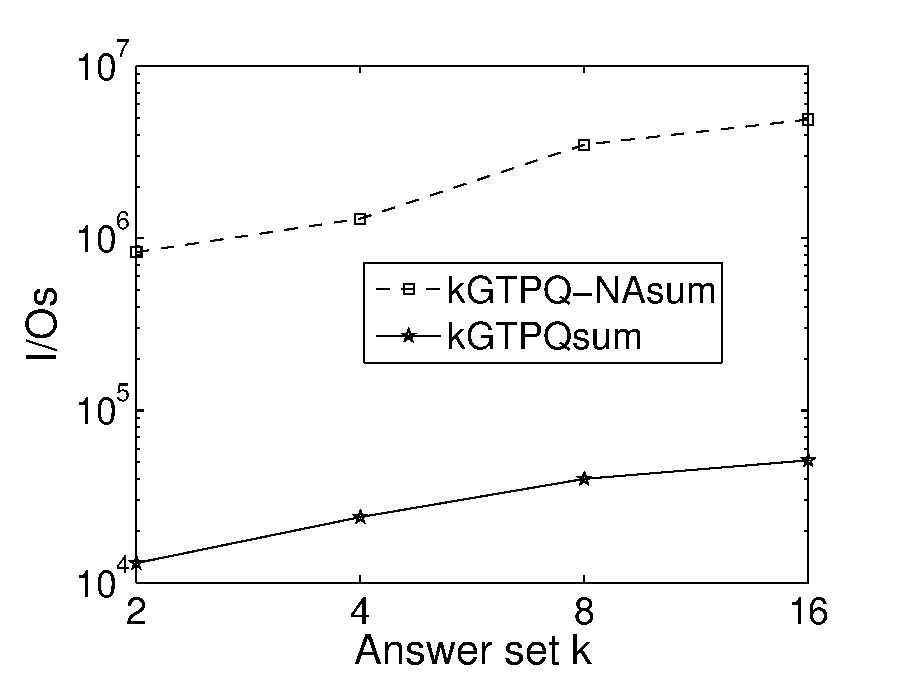
\includegraphics[]{graph/SumKIO.eps}} &
     %   \hspace{-5mm}
      %   \vspace{-2mm}
      %\resizebox{70mm}{!}{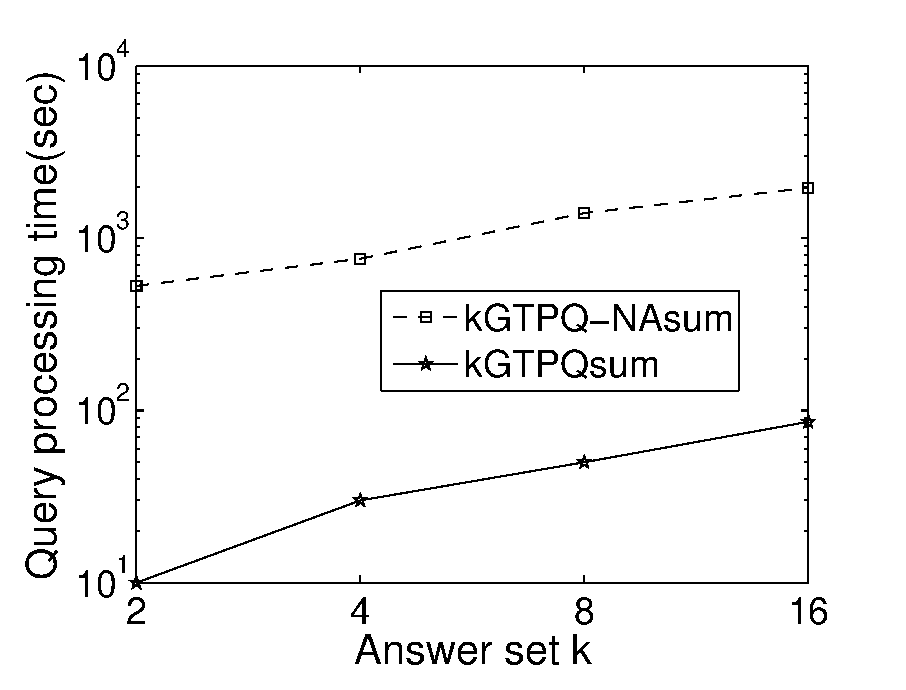
\includegraphics[]{graph/SumKTime.eps}} \\
      %\scriptsize{(a) \textsc{}\hspace{0mm}} & \scriptsize{(b) \textsc{}}\\
        %\hspace{-5mm}
%        \resizebox{40mm}{!}{\includegraphics{graph/sum/vk_io.pdf}} &
%        \hspace{-5mm}
%      \resizebox{40mm}{!}{\includegraphics{graph/max/vk_io.pdf}} \\
%      \scriptsize{(c) \textsc{sum}\hspace{0mm}} & \scriptsize{(d) \textsc{max}}\\
%      \hspace{-5mm}
%      \resizebox{40mm}{!}{\includegraphics{graph/sum/vk_answer.pdf}} &
%        \hspace{-5mm}
%      \resizebox{40mm}{!}{\includegraphics{graph/max/vk_answer.pdf}} \\
%       \scriptsize{(e) \textsc{sum}\hspace{0mm}} & \scriptsize{(f) \textsc{max}}
       % \end{tabular}
   %\caption{Effect of answer set $k$ for California data (a) I/Os and (b) Query processing time}
   % \label{graph:sum_k}
  %\end{center}
   %\vspace{-6mm}
%\end{figure}
%\vspace*{10pt}

%\textbf{\emph{Effect of Query Area $M$: }}In this case, we vary the query area $M$ as 2\%, 4\%, 8\% and 16\% of the data space. Figure~\ref{graph:sum_m}(a) and ~\ref{graph:sum_m}(b) show I/Os and query processing time, required by $kGTPQ_{sum}$ and $kGTPQ-NA_{sum}$, respectively. Since we need to access more data points from $R$-trees of different data types for a larger $M$, both I/Os and processing time increase with the increase of $M$ for both approaches.


%Figure~\ref{graph:sum_m}(a) shows that $kGTPQ-NA_{sum}$ requires at least one and half orders of
%magnitude more I/Os than that of $kGTPQ_{sum}$. Similarly, Figure ~\ref{graph:sum_m}(b)
%shows that the processing time of $kGTPQ-NA_{sum}$ is on average one order of magnitude higher
%than that of $kGTPQ_{sum}$.


%\vspace*{10pt}
%\begin{figure}[htbp]
 %\vspace{-2mm}
 % \begin{center}
  %  \begin{tabular}{cc}
   %      \hspace{-5mm}
    %  \resizebox{70mm}{!}{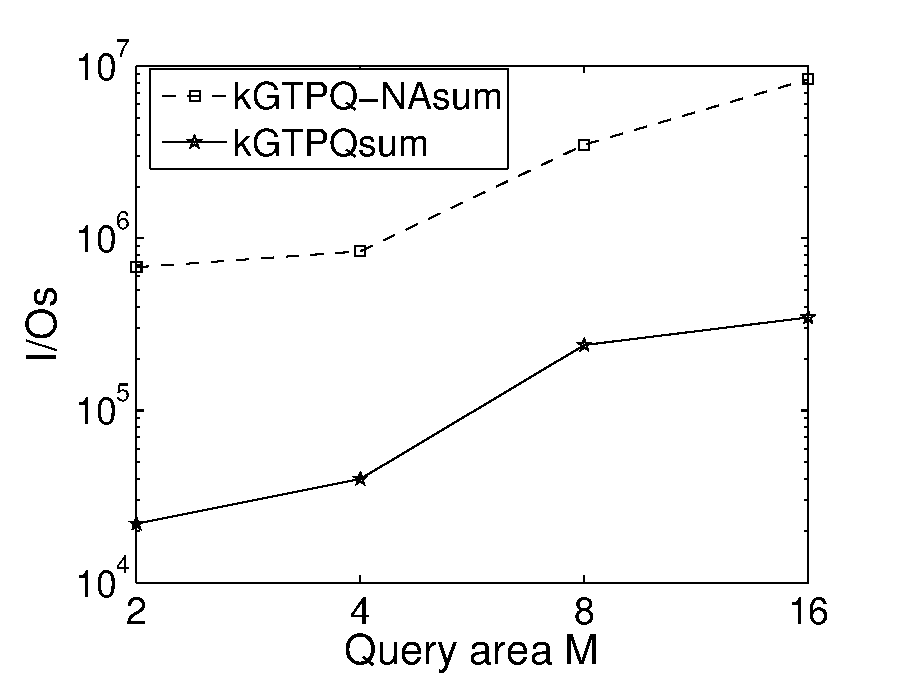
\includegraphics{graph/SumMIO.eps}} &
     %   \hspace{-5mm}
      %   \vspace{-2mm}
      %\resizebox{70mm}{!}{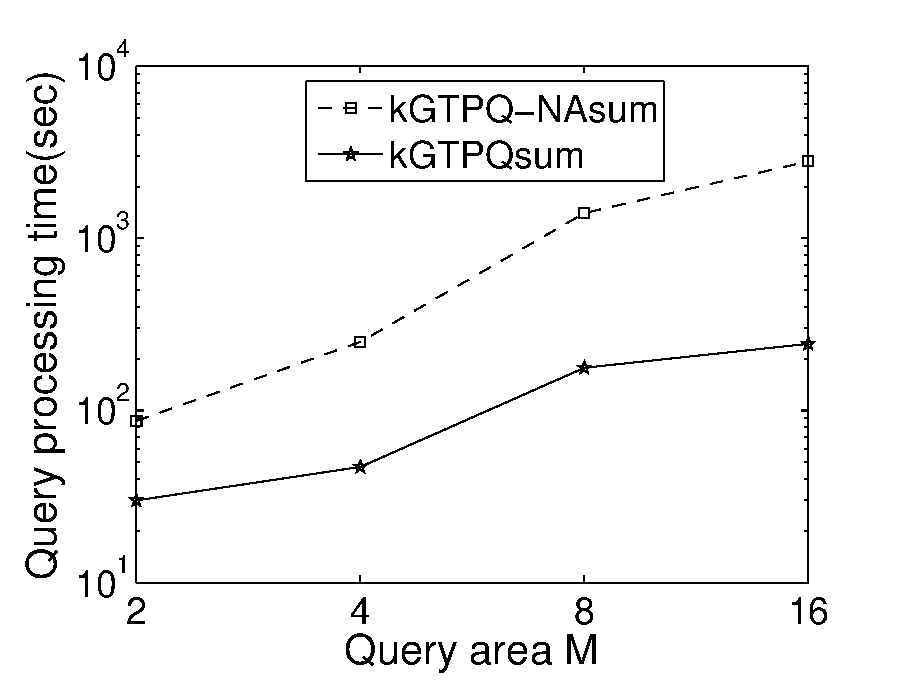
\includegraphics{graph/SumMTime.eps}} \\
      %\scriptsize{(a) \textsc{}\hspace{0mm}} & \scriptsize{(b) \textsc{}}\\
        %\hspace{-5mm}
%        \resizebox{40mm}{!}{\includegraphics{graph/sum/vk_io.pdf}} &
%        \hspace{-5mm}
%      \resizebox{40mm}{!}{\includegraphics{graph/max/vk_io.pdf}} \\
%      \scriptsize{(c) \textsc{sum}\hspace{0mm}} & \scriptsize{(d) \textsc{max}}\\
%      \hspace{-5mm}
%      \resizebox{40mm}{!}{\includegraphics{graph/sum/vk_answer.pdf}} &
%        \hspace{-5mm}
%      \resizebox{40mm}{!}{\includegraphics{graph/max/vk_answer.pdf}} \\
%       \scriptsize{(e) \textsc{sum}\hspace{0mm}} & \scriptsize{(f) \textsc{max}}
       %\end{tabular}
    %\caption{Effect of query area $M$ for California data (a) I/Os and (b) query processing time}
    %\label{graph:sum_m}
  %\end{center}
  % \vspace{-6mm}
%\end{figure}
%\vspace*{10pt}


%\textbf{\emph{Effect of dataset size: }}In this set of experiments, we vary the road network size and number of POIs as stated in Table~\ref{table:exp_synthetic}. In this case, we use the first column, i.e., varying the number of nodes as 5000,
%10000,15000 and 20000 to identify four synthetic datasets. Figure~\ref{graph:sum_u}(a)
%and ~\ref{graph:sum_u}(b) show I/Os and processing time respectively for
%different synthetic dataset sizes. As expected, the experimental results show that




\subsection{Our approach}
\label{subsec:max}

\endinput 